\documentclass[pdftex,letterpaper,10pt]{article}

\usepackage[bottom=3.25cm, top=3.25cm, left=2.0cm, right=2.0cm]{geometry}
\usepackage{fancyhdr}
\usepackage{graphicx}
\usepackage{hyperref}
\usepackage{tabulary}

\def\EmailAddress{name@domain.tld}
\def\PhoneNumber{555-555-5555}
\def\Name{Firstname Lastname}

\usepackage[bitstream-charter]{mathdesign}
\usepackage[T1]{fontenc}
\newcommand{\GitHubHeader}{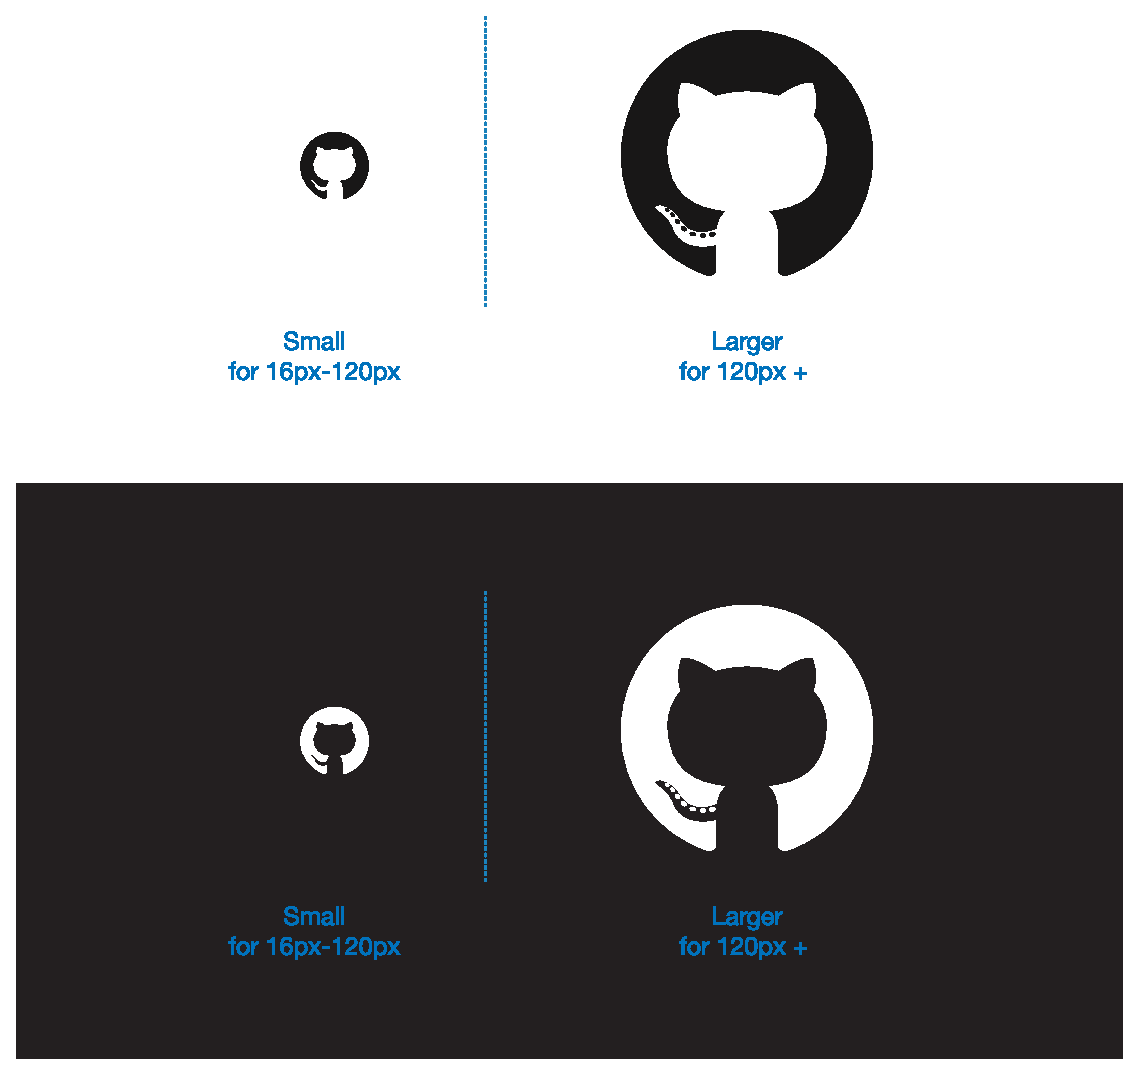
\includegraphics[clip,trim=4.8cm 14.55cm 12.75cm 1.95cm,scale=0.5]{img/GitHub-Mark.eps}}
\newcommand{\LinkedInHeader}{
\includegraphics[scale=0.4]{img/In-Black-0p5in-TM.eps}}

\newenvironment{skilltabular}{%
    \setlength\tabcolsep{3pt}%
    \setlength\parindent{0pt}%
    \renewcommand\arraystretch{1.25}%
    \noindent\tabulary{\textwidth}{@{}>{\bfseries}lL@{}}%
}
{\endtabulary}

\newenvironment{job}[1]{%
    \newenvironment{position}[2]{%
        \textit{##1} \hfill ##2%
        \begin{itemize}%
        \setlength\parskip\DetailParSkip%
    }{\end{itemize}}%
    \noindent\textbf{#1} \\%
}{}

\newenvironment{school}[1]{%
    \newenvironment{degree}[2]{%
        \textit{##1} \hfill ##2%
        \begin{itemize}%
        \setlength\parskip\DetailParSkip%
    }{\item[] \end{itemize} \vspace{-\dimexpr\baselineskip*3/2\relax}}%
    \noindent\textbf{#1} \\%
}{\vspace{-\dimexpr\baselineskip*2/3\relax}}


\fancyhead[L]{\EmailAddress}
\fancyhead[R]{\PhoneNumber}
\fancyhead[C]{\huge \bfseries \Name}

\pagestyle{fancy}

\renewcommand{\headrulewidth}{1.25pt}
\setlength{\headheight}{30pt}

\fancyfoot[C]{}

\begin{document}

\noindent
\begin{minipage}{\textwidth}
    \vspace{-30pt}
    \begin{minipage}{0.33\textwidth}
        \href{https://github.com/\GitHubUsername}{\raisebox{-.25\height}{\GitHubHeader} GitHub/\GitHubUsername}
    \end{minipage}
    \hfill
    \begin{minipage}{0.33\textwidth}
        \begin{center}
            \Address
        \end{center}
    \end{minipage}
    \hfill
    \begin{minipage}{0.33\textwidth}
        \raggedleft
        \href{https://www.linkedin.com/in/\LinkedInUsername}{\raisebox{-.25\height}{\LinkedInHeader} LinkedIn/\LinkedInUsername}
    \end{minipage}
\end{minipage}
\par\noindent\ignorespaces


\subsection*{Core Skills and Competencies}
\begin{skilltabular}
    General Skills  & Cooking, Cleaning, Organization \\
    Speaking Skills & Fast talking, Slow talking, Chipmunk talking, Foreign accents, Talking under my breath, Shouting, whining like a baby \\
    Others          & Eating lots of food all at once, Sleeping for 20 hours straight
\end{skilltabular}

\subsection*{Work Experience}
\begin{job}{Ministry of Silly Talks}
    \begin{position}{Talk Master}{June 2014 - Present}
        \item Talked to many unique individuals, mimicking their accents.
        \item Engaged in numerous speaking competitions on behalf of the company, winning dozens of prizes over the course of a few years, and earned top-speaker awards from the company itself.
        \item Convinced many high ranking individuals that I was a distinguished individual by using the right voices.
    \end{position}
    \begin{position}{Talk Instructor}{May 2013 - May 2014}
        \item Trained juniors how to talk silly talks.
        \item Helped other instructors create lesson plans for group session, and one on one sessions.
    \end{position}
\end{job}

\begin{job}{Sleep Center}
    \begin{position}{Junior Sleeper}{August 2012 - May 2013}
        \item Regularly trained in the sleeping arts.
        \item Once slept for 32 consecutive hours, when it was required to meet a quota from upper management.
    \end{position}
\end{job}

\end{document}
